\chapter{Datasets}
%
\label{chap:data}
%
\section{Data Collection}
%
We acquired data samples from patients referred to the Gastroenterology, Medical Oncology or Surgical outpatient departments (OPD) of the Postgraduate Institute of Medical Education and Research (PGIMER), Chandigarh (a tertiary care referral hospital in Northern India) for abdominal Ultrasound examinations of suspected \gb pathologies. The data was retrospective in nature, and consecutive patients with non-acute presentation were included in the study. The Ethics Committee of PGIMER approved the study. All procedures were performed according to the Declaration of Helsinki \footnote{The World Medical Association (WMA) developed the Declaration of Helsinki as the guiding ethical principle for medical research involving human subjects in 1964.} \cite{helsinki} and the research guidelines of The Indian Council of Medical Research (ICMR). We obtained informed written consent from the patients at the time of recruitment. We ensure the privacy of the patients by fully anonymizing the data. 

\par According to the hospital's protocol, overnight (or, at least 6 hours) of fasting was advised a day before the USG examinations for adequate distension of the GB. The radiologists at PGIMER Chandigarh performed the examinations on a Logic S8 machine (GE Healthcare) using a curved array low-frequency transducer (curvilinear probe type C1-5-D) with a frequency range of 1--5 MHz. We used the standard B-mode transabdominal USG for sample collection. Ultrasound scanning was done from different angles using both subcostal and intercostal views to visualize the entire GB, including the fundus, body, and neck. The scanning procedure intended to include the entire GB and the lesion or pathology. Patients were examined in different positions for adequate visualization of the GB. The screen area was adjusted so that the GB could occupy at least 20\% of the entire screen. We excluded color Doppler, spectral Doppler, annotations, and measurements. 

\par We have curated two different datasets for GBC detection -- image based, and video-based. The samples for these two datasets were collected from separate patient cohorts. For the image-based dataset, a minimum of 10 grayscale B-mode static images, including both sagittal and axial sections, were recorded by radiologists for each patient. For the video-based data, the entire USG scan for each patient was collected. We discuss the annotation and the statistics for both types of data in subsequent sections of this chapter. 

%\section{Dataset Collection and Curation}

%\myfirstpara{Data Collection}
%
%We acquired data samples from patients referred to PGIMER, Chandigarh (a tertiary care referral hospital in Northern India) for abdominal ultrasound examinations of suspected \gb pathologies. The study was approved by the Ethics Committee of PGIMER. We obtained informed written consent from the patients at the time of recruitment, and protect their privacy by fully anonymizing the data. Minimum 10 grayscale B-mode static images, including both sagittal and axial sections, were recorded by radiologists for each patient using a Logiq S8 machine. We excluded color Doppler, spectral Doppler, annotations, and measurements. Supplementary A %\ref{supp:data_collection} contains more details of the data acquisition process.
\section{Image-based Dataset}
\label{data:gbcu}
%
We call the image-based dataset as the Gallbladder Cancer Ultrasound (GBCU) dataset, and have publicly released it as a part of our published work \cite{basu2022surpassing}. We used the image-based dataset for developing and assessing various DNN models of GBC detection from USG images in Chapters \ref{chap:gbcnet}, \ref{chap:limited}, and \ref{chap:radformer}. 

\begin{figure}[t]
    \centering
     \begin{subfigure}[b]{0.3\linewidth}
		\centering
		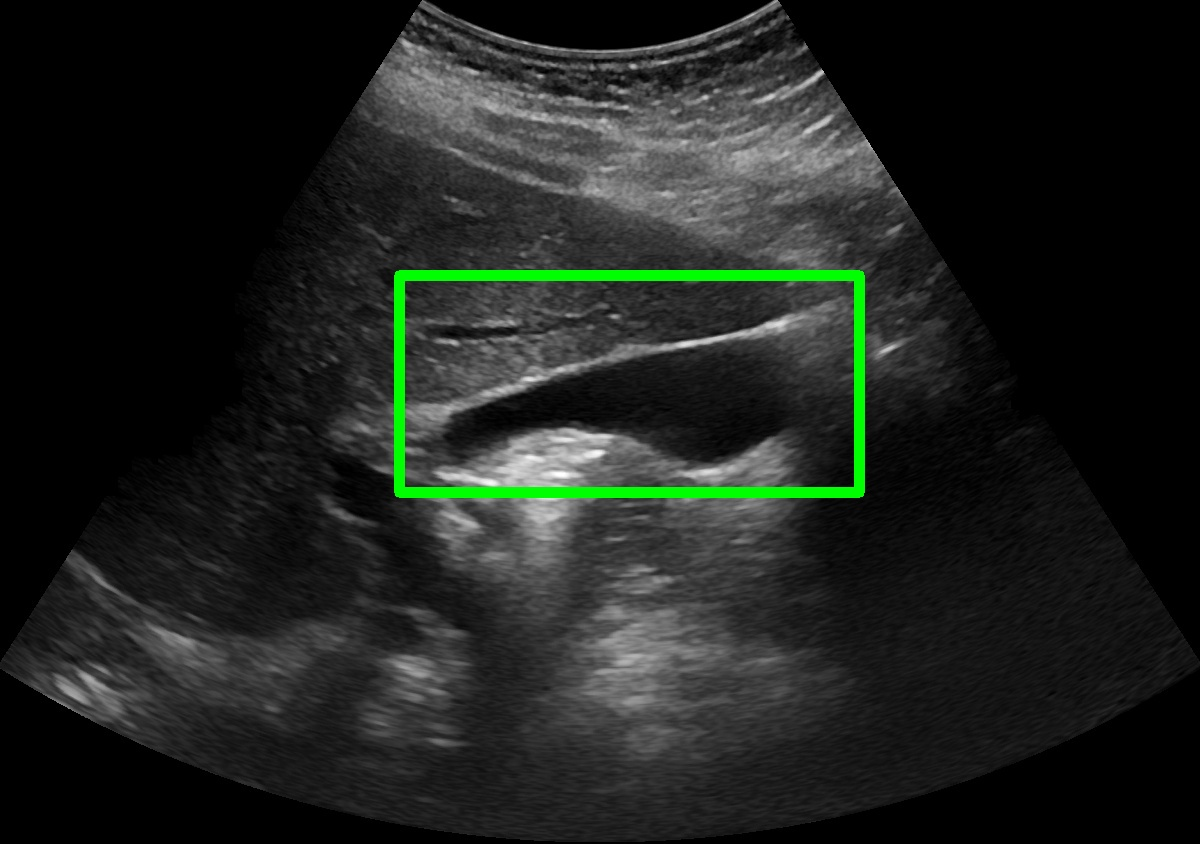
\includegraphics[width=\linewidth,height=10em]{figs/gbcnet/bbs-nml.png}
		\caption{}
	\end{subfigure}
    \begin{subfigure}[b]{0.3\linewidth}
		\centering
		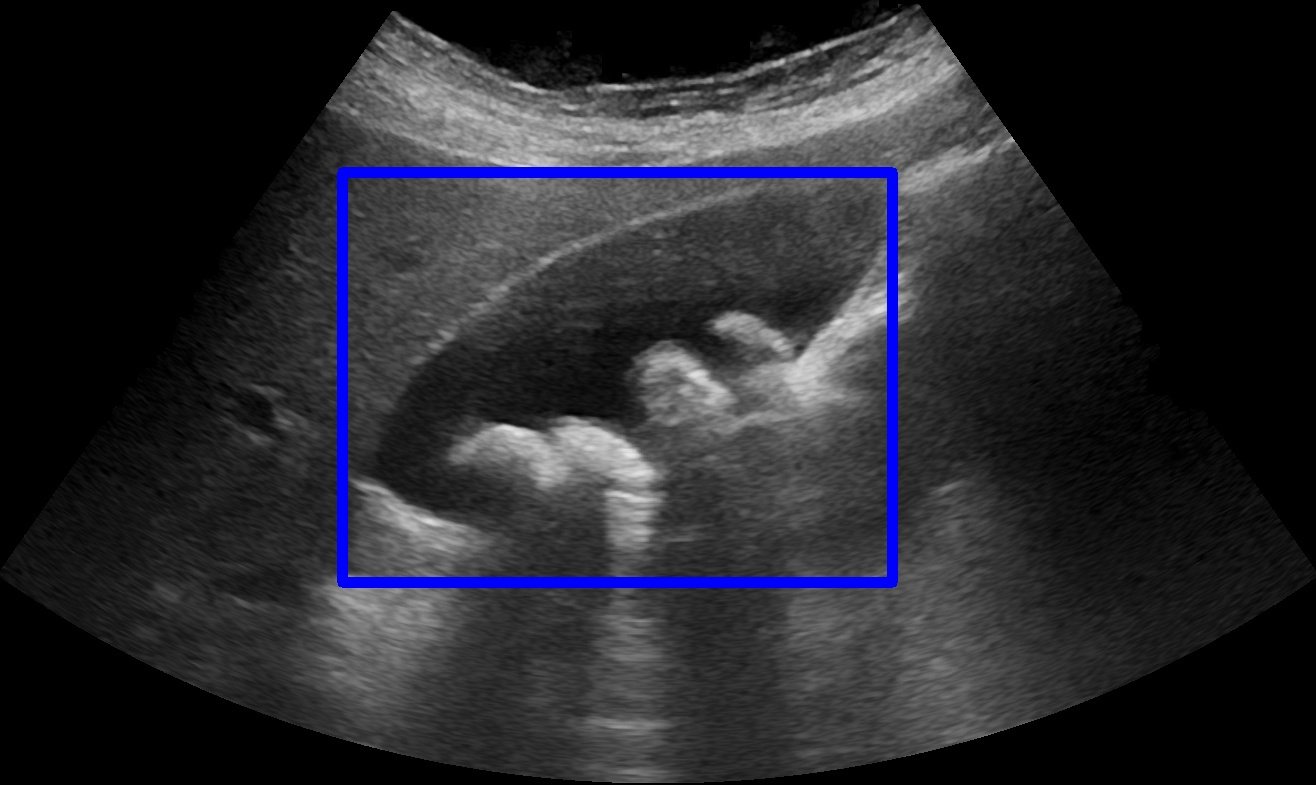
\includegraphics[width=\linewidth,height=10em]{figs/gbcnet/bbs-ben.png}
		\caption{}
	\end{subfigure}
    \begin{subfigure}[b]{0.3\linewidth}
		\centering
		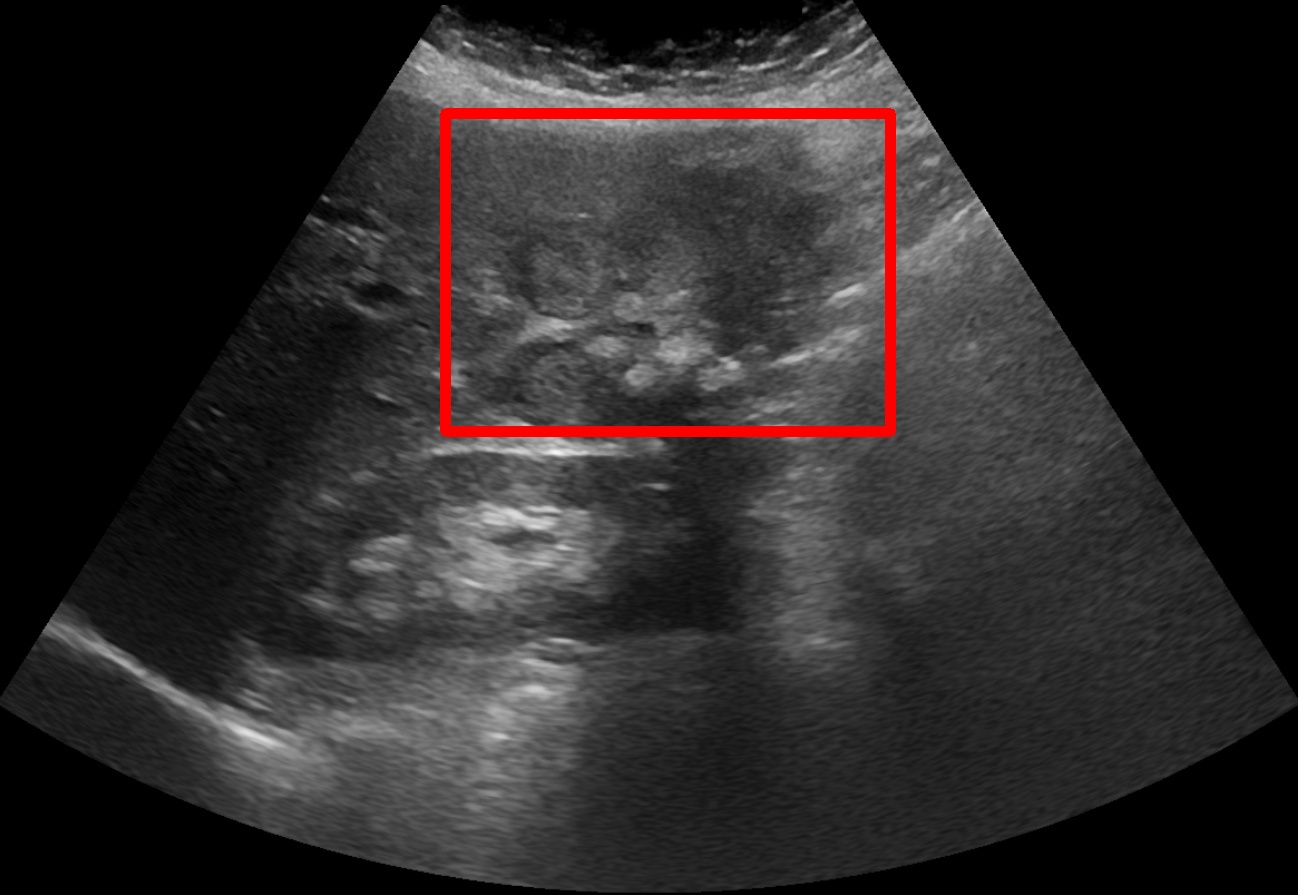
\includegraphics[width=\linewidth,height=10em]{figs/gbcnet/bbs-mlg.png}
		\caption{}
	\end{subfigure}
   \caption[Sample ROI annotation in USG images]{Sample ROI annotation. (a) Normal GB with ROI annotated in green, (b) GB with benign abnormalities with ROI in blue, and (c) Malignant GB with ROI annotated in red. }
    \label{fig:bb_sample}
\end{figure}
%
\subsection{Labeling and ROI Annotation}
%
Each image is labelled as one of the three classes - normal, benign, or malignant. These ground-truth classification labels were biopsy-proven to assert the correctness. Apart from image classification labels, we collected bounding-box annotations to capture the GB localization. Two expert radiologists with 10 and 2 years of experience in abdominal radiology did the bounding box labelling with consensus. Our radiologists used the LabelMe \cite{russell2008labelme} software to draw bounding boxes in the USG images of the dataset. In each image, the expert radiologists have drawn a single free-size axis-aligned bounding box spanning the entire \gb and adjacent liver parenchyma, preferably keeping the GB in the box's center to annotate the region of interest (\roi). \cref{fig:bb_sample} shows the sample \roi annotations drawn by the radiologists. For malignant cases, the \roi includes the visible malignant pathologies such as lesions, intraluminal polyp, mass, or malignant \gb wall thickening. 
%For the cases with no abnormality of the GB, the \roi contains the entire \gb. 

%\par In addition to the \roi, for the pathological GB cases, the %pathology was further highlighted using additional bouding boxes. Benign pathologies such as stones, benign wall thickening, benign polyp, sludge, and 
%regions containing the malignant pathologies such as lesion, intraluminal polyp, mass, or malignant \gb wall thickening were highlighted using axis-aligned bounding boxes covering only the pathological segment of the \gb. In the case of multiple anomalies in a single image, multiple boxes were drawn. 

\subsection{Dataset Statistics}
%
We have annotated 1255 abdominal \usg images collected from 218 patients from the acquired image corpus. Our dataset contains 71 patients with a normal gallbladder, 100 patients with benign abnormality, and 47 patients with malignancy. Overall, we have 432 normal, 558 benign, and 265 malignant images. The width of the images was between 801 and 1556 pixels, and the height was between 564 and 947 pixels. The variable size is due to cropping out of patient information from the Ultrasound image.

\subsection{Dataset Splits}
%
The sizes of the training and testing sets are 1133 and 122, respectively. To ensure generalization to unseen patients, all images of any particular patient were either in the train or the test split. The number of normal, benign, and malignant samples in the train and test set is 401, 509, 223, and 31, 49, and 42, respectively. Additionally, given the relatively small dataset, we report the 10-fold cross-validation metrics on the entire dataset for various experiments to assess generalization. All images of any particular patient appeared either in the training or the validation split during the cross-validation to guarantee the generalization to unseen patients.

% \begin{figure}
%     \centering
%     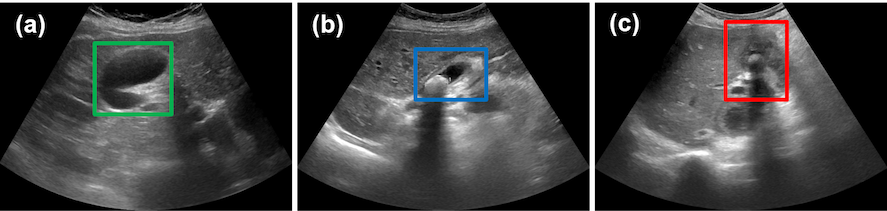
\includegraphics[width=\linewidth]{figs/radformer/annot-sample.png}
%     \caption{Sample ROI annotation. (a) Normal gallbladder with ROI in green, (b) benign GB with ROI in blue, and (c) malignant GB with ROI in red. }
%     \label{fig:data_sample}
% \end{figure}
%
%% DATASET
% \section{Dataset}
% %
% We have used the Gallbladder Cancer Ultrasound (GBCU) dataset \cite{basu2022surpassing}, publicly released by us in our previous work. For completeness, we provide a comprehensive description of the dataset in this section.

% \subsection{Data acquisition}
% %
% The patient data samples were acquired from the radiology department of the Postgraduate Institute of Medical Education \& Research (PGIMER, India). The patients were advised 8--8 hours of fasting before the examination for the adequate distension of the gallbladder. A Logic S8 machine (GE Healthcare) with a convex low-frequency transducer with a frequency of 1--5 MHz was used to capture the USG images. Radiologists having expertise in abdominal radiology assessed the patients from various positions and angles using subcostal and intercostal views for adequate visualization of the entire gallbladder, including its fundus, neck, and body. 
% A minimum of 10 Grayscale B-mode static images, including both sagittal and axial sections, were recorded for each patient.
% Colour Doppler, spectral Doppler, annotations, and measurements from the dataset are excluded. All personal textual information was removed from the images to anonymize them. 

% \subsection{Ground-truth labeling}
% %
% The biopsy reports of the patients are used to label each USG image as one of the three classes - normal, benign, or malignant. \radformer uses only these image-level labels during training. Apart from the image-level class labels, the bounding box annotations to locate the gallbladder and the surrounding ROI are also captured. It is important to note that we do not use these ROI bounding boxes during the training or inference of \radformer. 
% Two radiologists with 8 and 3 years of experience in abdominal radiology annotated the ROIs with consensus by using a single free-size axis-aligned box spanning the gallbladder and the adjacent regions. \cref{fig:data_sample} shows sample ROI annotations.

% \subsection{Statistics}
% %
% From the collected image corpus, the radiologists labeled 1255 USG images acquired from 218 patients. Our dataset contains 71 patients with a normal gallbladder, 100 patients with benign abnormality, and 47 patients with malignancy. Overall, the dataset contains 432 normal, 558 benign, and 265 malignant images. The images have a width of 801--1556 pixels and a height of 564--947 pixels. The variable size is due to cropping out of patient information from the image.

% \subsection{Dataset splits}
% %
% Given the relatively small dataset, we report 10-fold cross-validation metrics for various experimental models on the entire dataset. All images of any particular patient appeared either in the training or the validation split during the cross-validation to guarantee the generalization to unseen patients. Additionally we discuss the comparison with human experts using the GBCU test split containing 122 images (31 normal, 49 benign, and 42 malignant).


% subsection{In-house US Dataset for Gallbladder Cancer}
% %
% The transabdominal US video dataset is acquired at the Postgraduate Institute of Medical Education and Research (PGIMER), Chandigarh, India. The PGIMER ethics committee approved the study.

\section{Video Data}
\label{data:gbusv}
%
\subsection{Collection and Curation}
We have curated the video data in two phases. In the first phase, we collected 32 malignant and 32 non-malignant videos containing a total of 12,251 and 3,549 frames, respectively. 
%Radiologists with 2-8 years of experience in abdominal sonography acquired the data. The US videos were obtained after at least 6 hours of fasting using a 1--5 MHz curved array transducer (C-1-5D, Logiq S8, GE Healthcare). The scanning intended to include the entire GB and the lesion or pathology. The frame rate was 29 fps. 
%Note that we do not use video-level labels in our setup. 
We cropped the video frames from the center to anonymize the patient information and annotations. The processed video frames were of size $360\!\times\!480$ pixels. \cref{usucl_fig:data_sample} shows some samples from the video data. We have released this large-scale video dataset for the community as a part of our published work \cite{basu2022unsupervised}. We call this dataset Gallbladder Ultrasound Video (GBUSV) dataset. GBUSV was primarily used for the unsupervised contrastive pretraining for GBC representation learning discussed in \cref{chap:limited}. The video labels were not used during the contrastive pretraining.

% \mypara{Image Data}
% %
% We use the publicly contributed GBCU dataset \cite{basu2022surpassing} consisting of 1255 US images from 218 patients. The dataset consists of 990 non-malignant (171 patients with normal and benign GB) and 265 malignant (47 patients) GB images. The images were labeled as normal, benign, or malignant, and such labels were biopsy-proven. We use this dataset for finetuning and report 10-fold cross-validation. 
% %We did the cross-validation splits at the patient level, and all images of any patient appeared either in the train or validation split. 
% Note that the patients recorded in the video dataset are not included in this image dataset to ensure generalization. 


\begin{figure}[t]
    \centering
    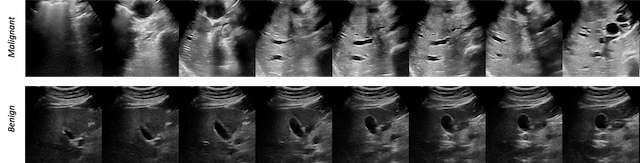
\includegraphics[width=\linewidth]{figs/focusmae/us_video.png}
    \caption[Video data samples]{Sample video sequences from our US video dataset used for GBC detection. We show samples of both malignant and benign (non-malignant) sequences for GBC video data. }
    \label{fig:video_data_sample}
\end{figure}

% 
In the second phase, we utilized the public GBUSV dataset and extended it with an additional set of USG videos collected by our team of radiologists. The extended dataset was used for developing and assessing video-based GBC detection models discussed in \cref{chap:focusmae}. We relied on the biopsy reports of the patients for labelling the videos. The GBUSV dataset comprises 64 Gallbladder US videos, with 32 labelled as benign and another 32 labelled as malignant. We added 27 additional US videos specifically depicting Gallbladder malignancy to the GBUSV dataset for curating the video dataset suitable for the video-based \gbc detection task. 
\cref{fig:video_data_sample} shows two sample video sequences, one belonging to a malignant patient, and the other collected from a patient with non-malignant \gb.
%We obtained video samples from patients referred to a tertiary care referral hospital for abdominal US examinations targeting suspected Gallbladder pathologies. Each patient provided informed written consent during recruitment, and we ensure patient privacy by fully anonymizing the data. The institute Ethics Committee approved the study. Patients were fasting for a minimum of 6 hours to ensure adequate distention of the \gb. Our team of radiologists employed a 1-5 MHz curved array transducer (C-1-5D, Logiq S8, GE Healthcare) for the scanning process. The scanning protocol covers the entire gallbladder (including fundus, body, and neck) and any associated lesions or pathologies. We cropped the video frames from the center to safeguard patient privacy and annotations. The processed frames have a size of 360x480 pixels. \cref{focusmae_fig:data_sample} shows sample sequences from the dataset. 

%\subsection{Annotation}
%%
%We relied on the GB biopsy reports for labeling the videos. %Additionally, two radiologists with 2 and 10 years of expertise in abdominal ultrasound (US), were consulted to draw bounding boxes covering the entire GB and the adjacent liver parenchyma in the frames where malignant lesion is visible. 
%The radiologists were pinpoint frames exhibiting clinical signs of malignancy. 
%In cases of malignant videos, the radiologists reached a consensus to label each frame as either malignant or non-malignant. 
%Although these frame-level annotations aren't directly employed for training video-based detection methods, they play a crucial role in qualitatively assessing the detectors. Moreover, these annotations hold potential for frame-level Video Anomaly Detection tasks. 
%Additionally, in each video, the radiologists have drawn an axis-aligned bounding box covering the entire GB and adjacent liver parenchyma to annotate the Region-of-Interest (ROI) that may contain the malignancy.

\subsection{Dataset Statistics}
%
The video dataset comprises 59 malignant and 32 non-malignant videos, collected from 41 malignant and 32 benign patients, respectively. The length of the videos varied from 43 to 888 frames. In total, the dataset encompasses 21,955 frames, with 18,406 frames attributed to videos labelled as malignant and 3,549 frames attributed to benign (non-malignant) videos. %Among these, radiologists identified 3212 frames exhibiting definite signs of malignancy. 

\subsection{Dataset Splits for Video-based GBC Detection}
%
We use the 5-fold cross-validation for the complete video dataset for key experiments in the video-based detection task. The cross-validation splits were conducted on a patient-wise basis, ensuring that all videos of a particular patient appeared exclusively in either the training or the validation split during cross-validation. Recall that the original GBUSV video dataset collected in the first phase did not contain any splits.